% Lab 3 Report - Full Subtractor Implementation
\documentclass[a4paper,12pt]{article}
\usepackage{graphicx}
\usepackage{listings}
\usepackage{hyperref}
\usepackage{geometry}
\usepackage{xcolor}
\usepackage{amsmath}
\geometry{left=1in, right=1in, top=1in, bottom=1in}

\lstset{
    frame=single,
    numbers=left,
    numberstyle=\tiny,
    basicstyle=\ttfamily\small,
    keywordstyle=\color{blue},
    commentstyle=\color{cyan},
    stringstyle=\color{red},
    breaklines=true,
    backgroundcolor=\color{gray!10}
}

\title{Lab Report\\ CSE4010 Computer Architecture}
\author{}
\date{}

\begin{document}

\maketitle

\noindent \textbf{Name:} \underline{Zachary A. Hampton\hspace{5cm}} \hfill \textbf{Score:} \underline{\hspace{2cm}/10} \\
\textbf{Student ID:} \underline{008339494\hspace{6cm}} \hfill \textbf{Due:} \underline{02-23-2025} \\
\textbf{Lab:} \underline{Lab 3 - Full Adder and Full Subtractor Implementation\hspace{6cm}}

\section*{Report}
\begin{itemize}
    \item How can addition and subtraction of large numbers be performed by computers if they are only aware of numbers 0 and 1?
    \begin{itemize}
        \item Computers perform arithmetic operations on large numbers by breaking them down into binary digits and processing them one bit at a time. For multi-digit numbers:
        \begin{itemize}
            \item Addition is performed using full adders in cascade, where each full adder processes one bit position and handles the carry from the previous stage
            \item Subtraction is similarly performed using full subtractors in cascade, where each subtractor handles one bit position and processes the borrow from the previous stage
            \item The carry/borrow propagation between stages allows for handling numbers of any size
        \end{itemize}
        \item This binary arithmetic is implemented using combinational circuits that:
        \begin{itemize}
            \item Process bits from least significant to most significant position
            \item Use carry/borrow propagation for managing digit transitions
            \item Can be extended to any number of bits by cascading multiple stages
        \end{itemize}
    \end{itemize}
\end{itemize}

\newpage

\section*{Source Code}
\subsection*{fullAdder.v}
\begin{lstlisting}[language=Verilog]
module fullAdder(
    input A,
    input B,
    input Cin,
    output sum,
    output Cout
);
    
    wire sum1, carry1, carry2;
    
    // First half adder
    assign sum1 = A ^ B;
    assign carry1 = A & B;
    
    // Second half adder
    assign sum = sum1 ^ Cin;
    assign carry2 = sum1 & Cin;
    
    // Final carry output
    assign Cout = carry1 | carry2;

endmodule
\end{lstlisting}

\newpage

\subsection*{fullAdder\_tb.v}
\begin{lstlisting}[language=Verilog]
`timescale 1ns/1ns
`include "fullAdder.v"

module fullAdder_tb;
    reg A, B, Cin;
    wire sum, Cout;
    
    fullAdder uut(
        .A(A),
        .B(B),
        .Cin(Cin),
        .sum(sum),
        .Cout(Cout)
    );
    
    initial begin
        $dumpfile("fullAdder_tb.vcd");
        $dumpvars(0, fullAdder_tb);
        
        // Test all input combinations
        A = 0; B = 0; Cin = 0; #20;
        A = 0; B = 0; Cin = 1; #20;
        A = 0; B = 1; Cin = 0; #20;
        A = 0; B = 1; Cin = 1; #20;
        A = 1; B = 0; Cin = 0; #20;
        A = 1; B = 0; Cin = 1; #20;
        A = 1; B = 1; Cin = 0; #20;
        A = 1; B = 1; Cin = 1; #20;
        
        $display("Test Complete!");
        $finish;
    end
    
    initial begin
        $monitor("Time=%0d A=%b B=%b Cin=%b sum=%b Cout=%b",
                 $time, A, B, Cin, sum, Cout);
    end
endmodule
\end{lstlisting}

\newpage

\subsection*{fullSubtractor.v}
\begin{lstlisting}[language=Verilog]
module fullSubtractor(
    input A,
    input B,
    input Bin,
    output diff,
    output Bout
);
    
    wire diff1, borrow1, borrow2;
    
    // First half subtractor
    assign diff1 = A ^ B;
    assign borrow1 = !A & B;
    
    // Second half subtractor
    assign diff = diff1 ^ Bin;
    assign borrow2 = !diff1 & Bin;
    
    // Final borrow output
    assign Bout = borrow1 | borrow2;

endmodule
\end{lstlisting}

\newpage

\subsection*{fullSubtractor\_tb.v}
\begin{lstlisting}[language=Verilog]
`timescale 1ns/1ns
`include "fullSubtractor.v"

module fullSubtractor_tb;
    reg A, B, Bin;
    wire diff, Bout;
    
    fullSubtractor uut(
        .A(A),
        .B(B),
        .Bin(Bin),
        .diff(diff),
        .Bout(Bout)
    );
    
    initial begin
        $dumpfile("fullSubtractor_tb.vcd");
        $dumpvars(0, fullSubtractor_tb);
        
        // Test all input combinations
        A = 0; B = 0; Bin = 0; #20;
        A = 0; B = 0; Bin = 1; #20;
        A = 0; B = 1; Bin = 0; #20;
        A = 0; B = 1; Bin = 1; #20;
        A = 1; B = 0; Bin = 0; #20;
        A = 1; B = 0; Bin = 1; #20;
        A = 1; B = 1; Bin = 0; #20;
        A = 1; B = 1; Bin = 1; #20;
        
        $display("Test Complete!");
        $finish;
    end
    
    initial begin
        $monitor("Time=%0d A=%b B=%b Bin=%b diff=%b Bout=%b",
                 $time, A, B, Bin, diff, Bout);
    end
endmodule
\end{lstlisting}

\section*{Screenshots}
\subsection*{Part A - Full Adder Simulation}
\begin{figure}[h]
    \centering
    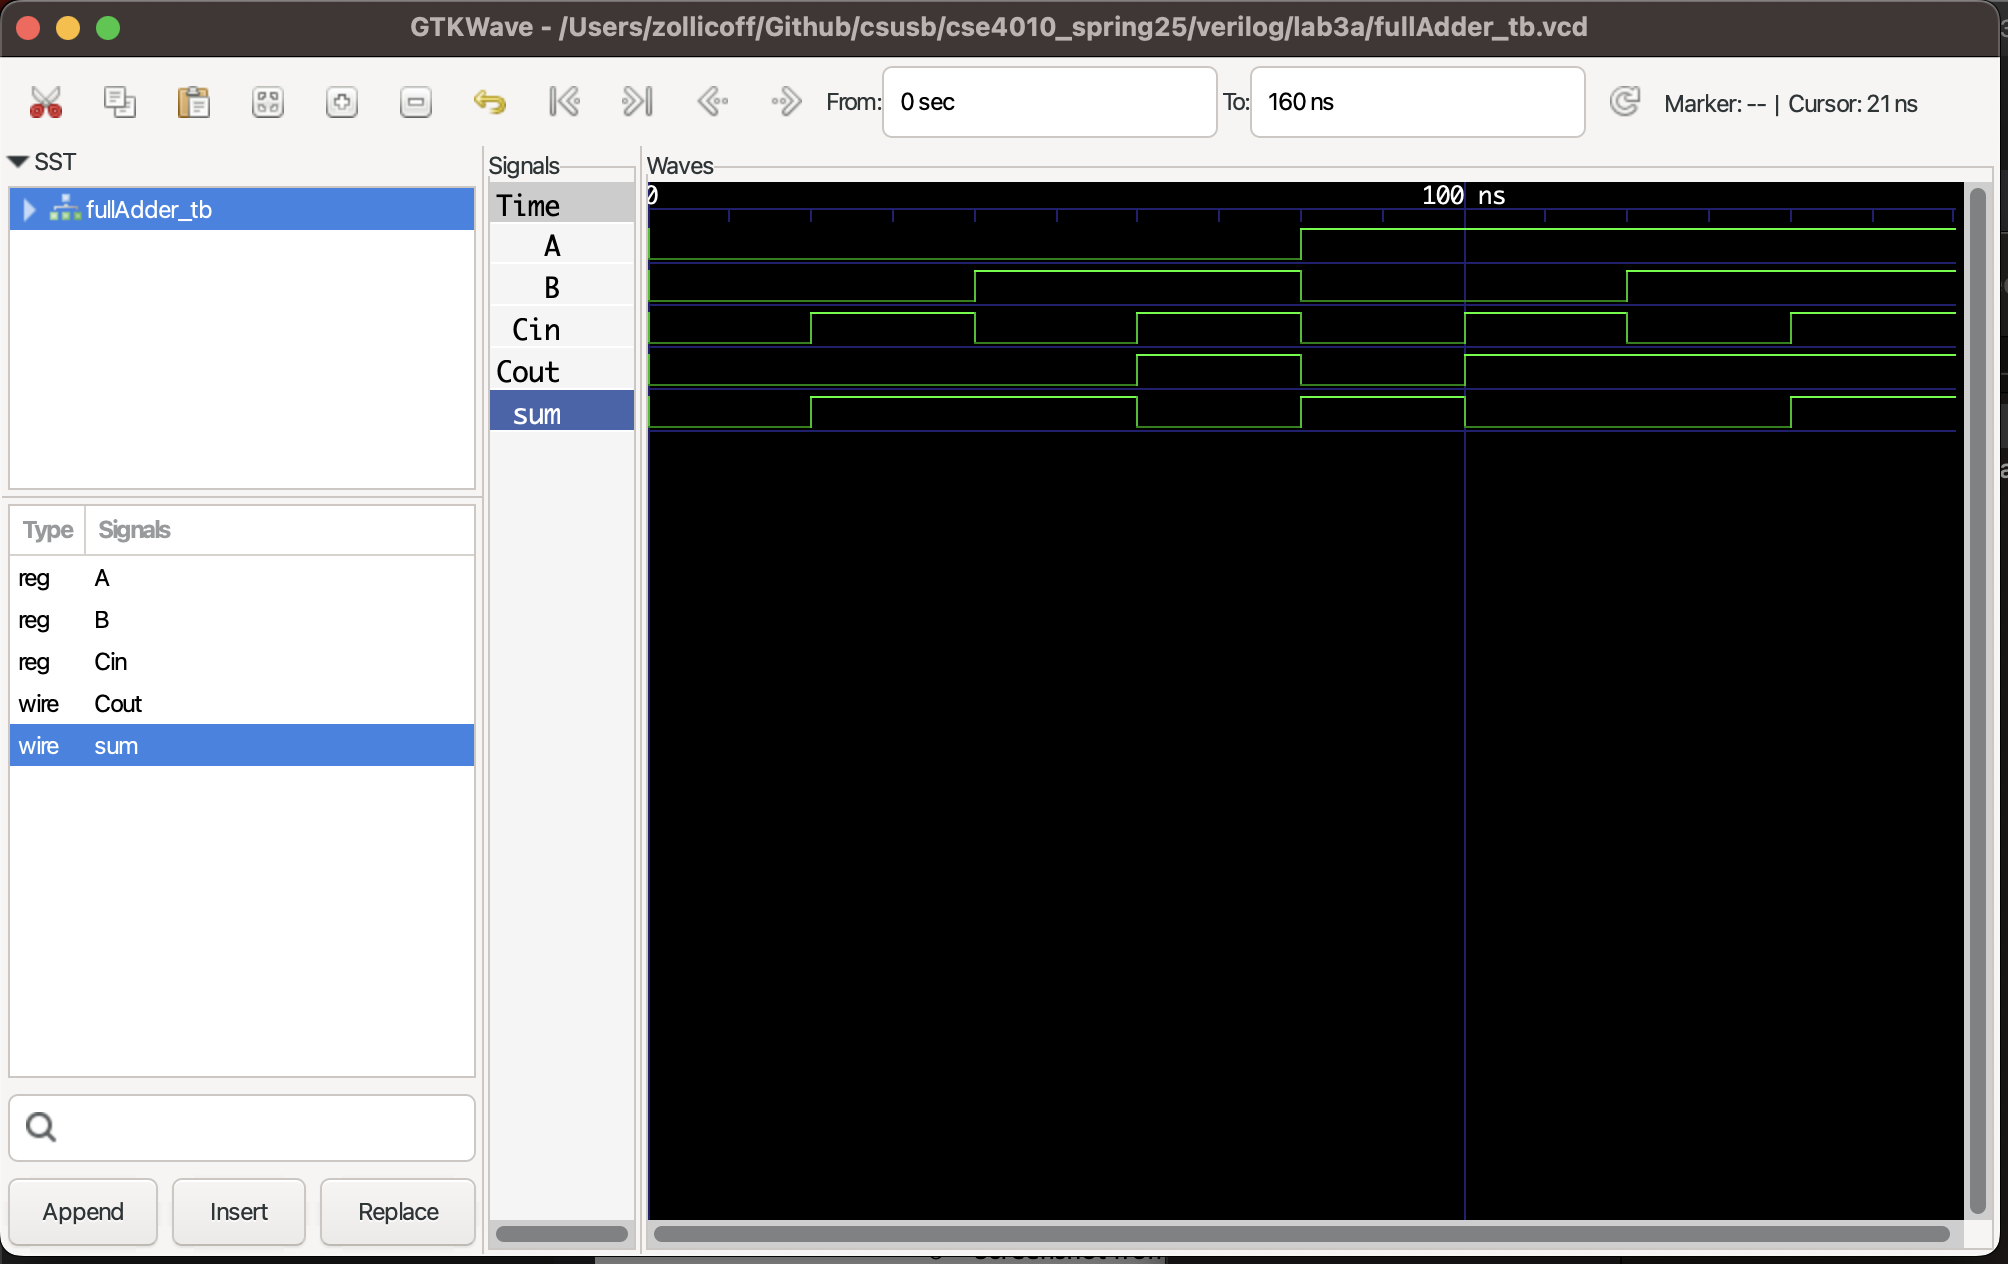
\includegraphics[width=\textwidth]{full_adder.png}
    \caption{Full Adder Simulation Waveform showing all test cases with inputs A, B, Cin and outputs sum, Cout}
\end{figure}

\subsection*{Part B - Full Subtractor Simulation}
\begin{figure}[h]
    \centering
    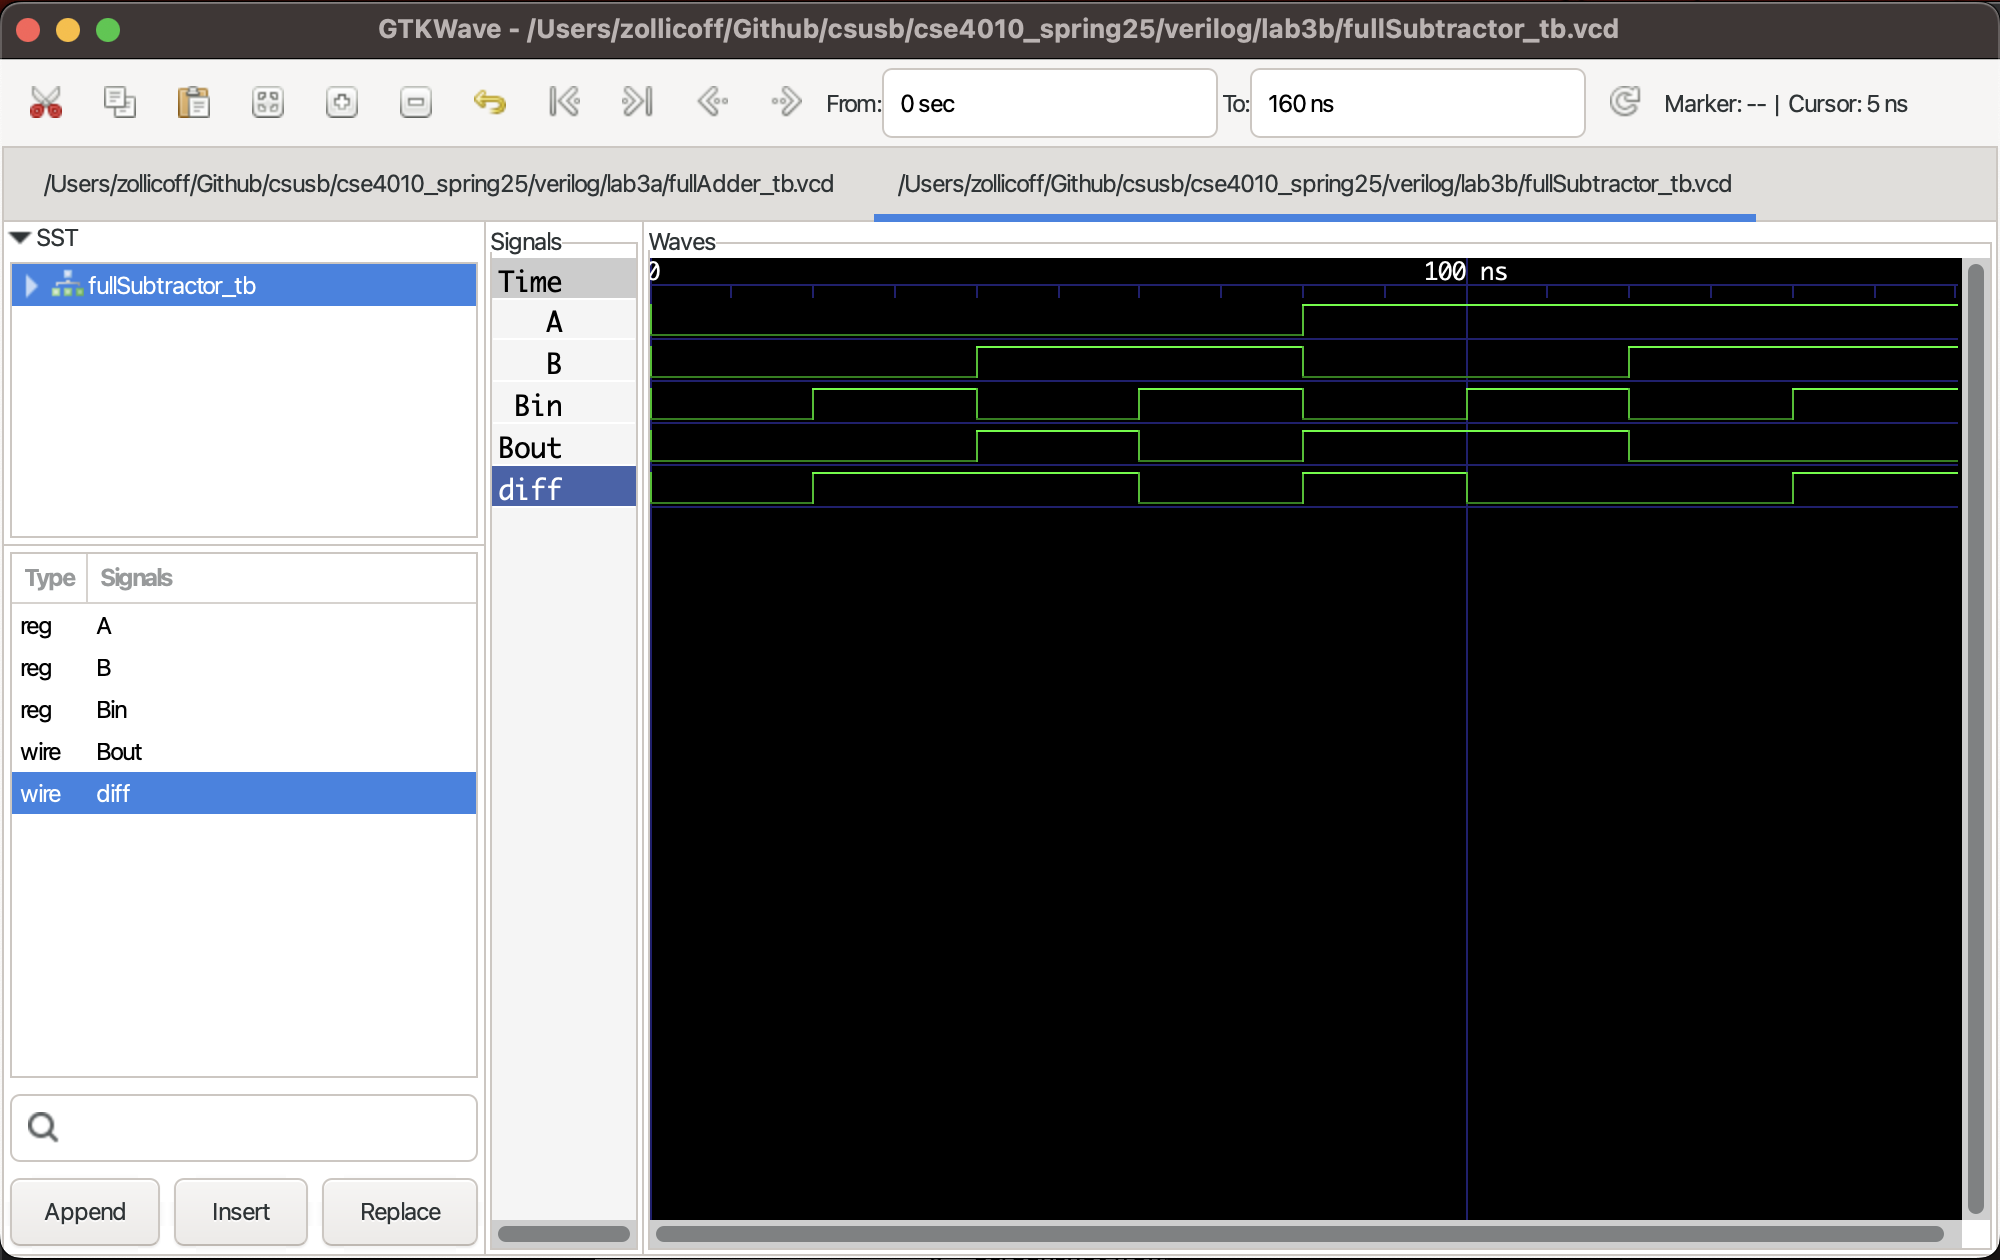
\includegraphics[width=\textwidth]{full_subtractor.png}
    \caption{Full Subtractor Simulation Waveform showing all test cases with inputs A, B, Bin and outputs diff, Bout}
\end{figure}

\end{document} 